\subsubsection{Évolution temporelle}

Pour étudier la dynamique temporelle de notre chaîne de Markov, nous calculons la distribution de probabilité des états au temps $t$, notée $u_t$. Si la chaîne possède un vecteur de probabilité initial $u_0$, la distribution au temps $t$ est donnée par l'équation :
\begin{equation}
    u_t = u_0 P^t
\end{equation}

Nous avons simulé cette évolution sur 20 étapes temporelles pour deux conditions initiales distinctes :
\begin{enumerate}
    \item Une distribution initiale uniforme : $u_0 = (0.25, 0.25, 0.25, 0.25)$.
    \item Un départ certain depuis le nucléotide 'C' : $u_0 = (0, 1, 0, 0)$.
\end{enumerate}

La Figure \ref{fig:evolution_markov} illustre les résultats obtenus.

\begin{figure}[ht]
    \centering
    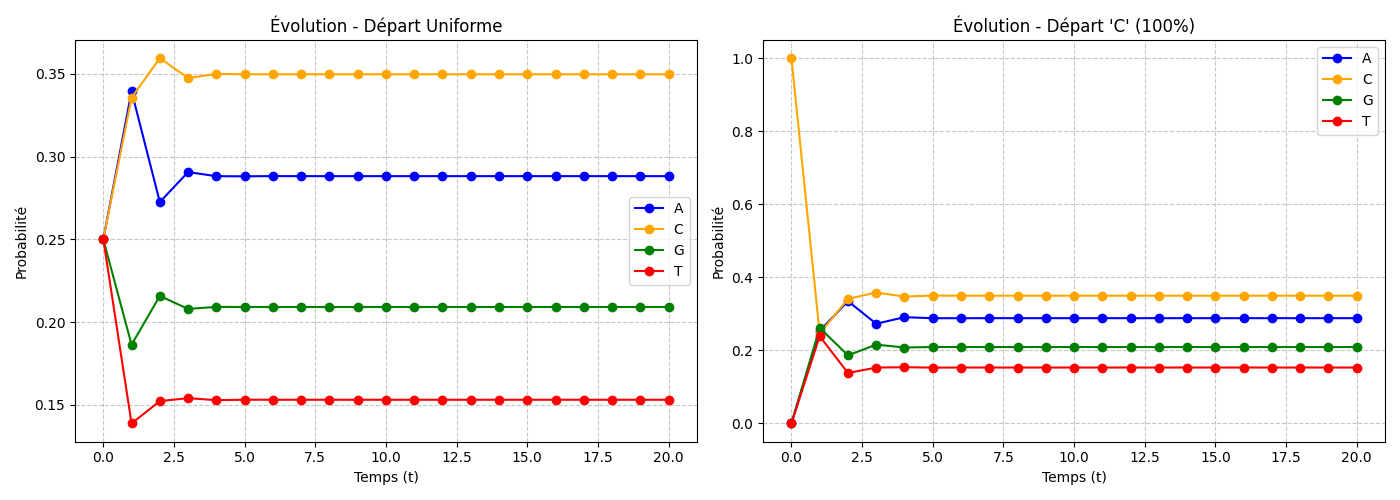
\includegraphics[width=1\textwidth]{images/evolution_markov.png}
    \caption{Évolution de la probabilité de se trouver dans chaque état (A, C, G, T) au cours du temps, pour deux conditions initiales différentes.}
    \label{fig:evolution_markov}
\end{figure}

\subparagraph{Analyse des observations}
Nous remarquons que, bien que les trajectoires des premières étapes 
soient très différentes selon la condition initiale, les probabilités 
finissent par se stabiliser et converger vers des valeurs constantes après 
environ $t = 3$ itérations. 

Indépendamment de la condition initiale, les probabilités convergent toutes vers le même ordre
$P(C) > P(A) > P(G) > P(T)$. Les différences observées lors des premières étapes (phase transitoire) 
disparaissent rapidement, démontrant que la chaîne « oublie » son point de départ en convergeant 
vers sa distribution stationnaire unique.

En calculant la matrice $P^t$ pour une valeur de $t$ suffisamment grande (par exemple $t=50$), nous observons le résultat suivant :
\begin{equation}
P^{50} \approx
    \begin{pmatrix}
        0.2881 & 0.3497 & 0.2091 & 0.1531 \\
        0.2881 & 0.3497 & 0.2091 & 0.1531 \\
        0.2881 & 0.3497 & 0.2091 & 0.1531 \\
        0.2881 & 0.3497 & 0.2091 & 0.1531
    \end{pmatrix}
\end{equation}

Les lignes de la matrice $P^t$ deviennent toutes identiques. 
Cela s'explique mathématiquement : l'élément $(i,j)$ de $P^t$ représente la probabilité 
de se trouver dans l'état $j$ après $t$ étapes en partant de l'état $i$. Le fait que toutes 
les lignes soient égales signifie que pour un temps $t$ suffisamment long, la probabilité 
d'être dans un état donné ne dépend plus du tout de l'état de départ. La chaine a "oublié" 
sa condition initiale lors qu'elle converge vers la distribution stationnaire.